\documentclass[10pt]{article}\usepackage[]{graphicx}\usepackage[]{xcolor}
% maxwidth is the original width if it is less than linewidth
% otherwise use linewidth (to make sure the graphics do not exceed the margin)
\makeatletter
\def\maxwidth{ %
  \ifdim\Gin@nat@width>\linewidth
    \linewidth
  \else
    \Gin@nat@width
  \fi
}
\makeatother

\definecolor{fgcolor}{rgb}{0.345, 0.345, 0.345}
\newcommand{\hlnum}[1]{\textcolor[rgb]{0.686,0.059,0.569}{#1}}%
\newcommand{\hlsng}[1]{\textcolor[rgb]{0.192,0.494,0.8}{#1}}%
\newcommand{\hlcom}[1]{\textcolor[rgb]{0.678,0.584,0.686}{\textit{#1}}}%
\newcommand{\hlopt}[1]{\textcolor[rgb]{0,0,0}{#1}}%
\newcommand{\hldef}[1]{\textcolor[rgb]{0.345,0.345,0.345}{#1}}%
\newcommand{\hlkwa}[1]{\textcolor[rgb]{0.161,0.373,0.58}{\textbf{#1}}}%
\newcommand{\hlkwb}[1]{\textcolor[rgb]{0.69,0.353,0.396}{#1}}%
\newcommand{\hlkwc}[1]{\textcolor[rgb]{0.333,0.667,0.333}{#1}}%
\newcommand{\hlkwd}[1]{\textcolor[rgb]{0.737,0.353,0.396}{\textbf{#1}}}%
\let\hlipl\hlkwb

\usepackage{framed}
\makeatletter
\newenvironment{kframe}{%
 \def\at@end@of@kframe{}%
 \ifinner\ifhmode%
  \def\at@end@of@kframe{\end{minipage}}%
  \begin{minipage}{\columnwidth}%
 \fi\fi%
 \def\FrameCommand##1{\hskip\@totalleftmargin \hskip-\fboxsep
 \colorbox{shadecolor}{##1}\hskip-\fboxsep
     % There is no \\@totalrightmargin, so:
     \hskip-\linewidth \hskip-\@totalleftmargin \hskip\columnwidth}%
 \MakeFramed {\advance\hsize-\width
   \@totalleftmargin\z@ \linewidth\hsize
   \@setminipage}}%
 {\par\unskip\endMakeFramed%
 \at@end@of@kframe}
\makeatother

\definecolor{shadecolor}{rgb}{.97, .97, .97}
\definecolor{messagecolor}{rgb}{0, 0, 0}
\definecolor{warningcolor}{rgb}{1, 0, 1}
\definecolor{errorcolor}{rgb}{1, 0, 0}
\newenvironment{knitrout}{}{} % an empty environment to be redefined in TeX

\usepackage{alltt}

\usepackage{times}
\RequirePackage{natbib}
\usepackage[colorlinks=true, citecolor=blue, linkcolor=blue]{hyperref}
\usepackage{amsmath, amssymb, fullpage, amsthm, array, graphicx, asa, url}

\graphicspath{{images/}}

% JASA guideline to have double spaced fonts
\usepackage{setspace}
\doublespacing


\usepackage{color}
\definecolor{mahbub}{rgb}{1.0, 0.6, 0.4}

\newcommand{\hh}[1]{{\color{magenta} #1}}
\newcommand{\dc}[1]{{\color{green} #1}}
\newcommand{\mm}[1]{{\color{mahbub} #1}}
\renewcommand*\familydefault{\sfdefault} % To make font Halvatica, Wiley requirement

\setlength{\oddsidemargin}{0in}
\setlength{\evensidemargin}{0in}
\setlength{\textwidth}{6.5in}
\setlength{\topmargin}{-0.4in}
\setlength{\textheight}{9in}
\evensidemargin 
\oddsidemargin

\pdfminorversion=4 % as instructed by JASA file upload
% NOTE: To produce blinded version, replace "1" with "0" below. 
% Blinded version will also remove acknowledgement at the bottom.
\newcommand{\blindDoc}{1}
\IfFileExists{upquote.sty}{\usepackage{upquote}}{}
\begin{document}

% ===================================================================================
%Article top matter 
%------------------------------------------------------------------------------------

\if1\blindDoc
{
  \title{Effect of Sociological Factors on Visual Statistical Inference}
  \author{{Mahbubul Majumder, Heike Hofmann, Dianne Cook}
\thanks{Mahbubul Majumder is an Associate Professor in the Department of Mathematical and Statistical Sciences, University of Nebraska Omaha, NE 68182 (e-mail: mmajumder@unomaha.edu), Heike Hofmann is Professor in the Department of Statistics, University of Nebraska Lincoln, NE, and  Dianne Cook is Professor in the Department of Econometrics and Business Statistics, Monash University, Australia. This research is supported in part by the National Science Foundation Grant \# DMS 1007697.}}
\date{\vspace{-.5in}}
  \maketitle
} \fi

\if0\blindDoc
{
  \bigskip
  \bigskip
  \bigskip
  \begin{center}
    {\bf \LARGE Human Factors Influencing Visual Statistical Inference}
\end{center}
  \medskip
} \fi


% ===================================================================================
\begin {abstract} 
%------------------------------------------------------------------------------------

Visual statistical inference determines the significance of patterns found in data exploration through graphics. It involves human observers inspecting a lineup of plots, with one real data plot randomly placed among decoys. Each observer's cognitive skills and judiciousness can influence results. The effectiveness of this method, measured by power, depends on combining evaluations from multiple observers. Factors influencing power include observer demographics, visual skills, experience, the sample of null plots, plot position, and signal strength. This paper examines these factors through studies using Amazon's Mechanical Turk, finding individual skills vary but demographics have little impact. Learning increases speed but not accuracy, and plot position doesn’t affect results.

{\bf Keywords: \sf statistical graphics, non-parametric test, cognitive psychology, data visualization, exploratory data analysis, data mining, visual analytics.} 
\end {abstract}

% ===================================================================================
\section{Introduction}  
%------------------------------------------------------------------------------------

The lineup protocol introduced by \citet{buja:2009} quantifies the significance of graphical findings in exploratory data analysis, forming part of visual statistical inference. \citet{majumder:2013} extended and validated this approach through simulation studies, showing that visual inference can sometimes outperform conventional methods. They also defined the power of visual tests and proposed a way to calculate it for a given lineup. In visual inference, the test statistic is a plot of observed data, randomly placed among null plots generated under a null hypothesis, often assuming no structure. Observers evaluate the lineup, and if they consistently identify the data plot, this provides evidence against the null hypothesis, akin to a conventional hypothesis test.

A lineup can be evaluated by one or more observers, and a distribution similar to the binomial, adjusted for dependencies from the lineup scenario, is used to calculate the $p$-value based on how often the actual data plot is identified \citep{vinference}. To avoid expectation bias \citep{meilgaard}, observers must not know the data constituting the lineup or have seen the actual data plot beforehand. The accompanying question in a lineup should be broad, asking observers to pick the most distinct plot, allowing detection of any deviations from the null hypothesis. However, in head-to-head tests with conventional methods \citep{majumder:2013, tengfei:2013}, specific questions are needed to avoid type III errors \citep{mosteller:48} consisting of correctly rejecting the null hypothesis for a wrong reason.

The lineup protocols allows us to calculate all relevant properties that we are familiar with from conventional statistical tests. In particular, the power of a lineup is calculated as the {\it detection rate} at which observers identify the actual data plot. Visual power depends unlike power in conventional tests not only on the strength of the signal, but also on individuals' ability. The ability of individual observers varies, and the effects that might influence this ability are the focus of this paper.

We conducted several experiments (see Table~\ref{tbl:visual_stat} in the Appendix~\ref{sec:tbl_fig}) using Amazon's Mechanical Turk~\citep{turk} (MTurk) for validating the lineup protocol, comparing plot designs, and evaluating data analysis structures. Demographic data such as gender, age, and educational background were collected to assess the influence of these covariates on lineup evaluations. Additionally, experiments investigated the short-term learning trends.

Section~\ref{sec:factor_performance} discusses expected human factors influencing observer performance and Section~\ref{sec:result_socio} presents findings on factors affecting lineup evaluations. The methods used to assess the effects are oulined in Appendix~\ref{sec:exp_design}. 



% ===================================================================================
\section{Factors Potentially Affecting Visual Inference} \label{sec:factor_performance} 
%------------------------------------------------------------------------------------

Visual statistical inference relies not only on the strength of the signal in the data, but also on how this information is presented in the plot, on the lineup design and on the abilities of human observers. It is important to understand how these factors might affect results.  Here, we provide a brief discussion %This section provides a brief description 
of the factors that are expected to have some impact on the performance of visual statistical inference.  


\begin{itemize} \itemsep 0in \parsep-10pt %\parskip0pt 
 
\item{\bf Demographics:}  During each of the experiments, data on age, gender, education level and geographic location was collected. Each observer self-reported gender, age in roughly five year intervals, education level as high school or less, some college courses, an undergraduate degree, some graduate courses or a graduate degree. The IP address of the computer afforded the geographical location of the subject.

\item{\bf Learning Trend:} One might expect that as an observer evaluates more lineups they  become more skillful in their evaluations. Each participant in  experiments~5, 6 and~7 was asked to evaluate a block of  ten lineups of the same type of data plot. The ten lineups were randomly chosen from the lineups  produced for each study. Before evaluating the first lineup, the observer needs to read instructions and become accustomed to the type of plot used in the lineup. In subsequent lineups  the type of plot is the same. It is possible that the observer becomes more skillful at recognizing the most different plot, either by more often detecting the actual data plot or more quickly reporting their choice. These two ways of measuring learning trend are evaluated on data collected from experiments~5, 6 and~7.


%\subsection{Individual Skill or Ability} 
\item{\bf Individual Skill or Ability:} Each person may have different  aptitude for reading statistical plots, and their visual skill sets might be differently developed.  We can examine the effect of individuals' skills and abilities because multiple subjects evaluated the same lineups, which allows us to estimate, if some subjects consistently detect the actual data plot more often than others.  

\end{itemize}



% ===================================================================================
\section{Results}\label{sec:result_socio}
%------------------------------------------------------------------------------------

 \subsection{Overview of the Data} In ten experimental studies, a total of 2,340 participants from 70 countries, primarily the United States and India, provided feedback data on lineups, ensuring a diverse pool of respondents in terms of geography, gender, age, and education. There were a high number of female participants(42\%) across most countries, which was an unexpected but positive outcome(see Table~\ref{tbl:turker_location} in Appendix~\ref{sec:tbl_fig}). Notably, countries like Canada, Romania, the United Kingdom, and Macedonia also had notable participant representation.

The majority of participants were aged 18 to 35, with the United States showing a more balanced age distribution compared to India, where younger individuals were more prevalent. Educational backgrounds were diverse, with 38.42\% of participants reporting a graduate degree. However, there was a cultural misunderstanding as Indian participants classified any university degree as a graduate degree, while the North American definition refers to a Master’s degree or higher. Compared to the 2010 US Census \cite{census}, the participants skewed younger and more highly educated.

A total of 1,912 lineups were evaluated across the studies, with each participant reviewing at least 10 lineups, except for experiment~9, where they reviewed three. To ensure quality, participants were given test plots to evaluate first, and incorrect responses led to their data being excluded from the analysis. Some demographic and geographical data were missing due to participants opting out or issues retrieving IP-based location data.


\subsection{Demographic Factors} 

To explore the significance of demographic factors in detecting the data plot in the lineup, a mixed-effects model~\eqref{eqn:demographic_response} is fitted to the data, with age, country, education, and gender as fixed effects. To estimate the significance of each of the factors, reduced models are fitted with that factor removed from the model. Table~\ref{tbl:model_result_demographics} summarizes the results. Except for gender, all of the demographic factors show significant differences in  detection rates.  With respect to time taken, all of the demographic factors are significant. 


% latex table generated in R 3.4.1 by xtable 1.8-2 package
% Wed Oct 18 17:22:24 2017
\begin{table}[hbtp]
\caption{\label{tbl:model_result_demographics}Parameter estimates of models~\eqref{eqn:demographic_time} and~\eqref{eqn:demographic_response} fitted for average log time taken and detection rate, respectively. For time taken all the demographic factors are significant. For detection rate, age group 36-40, rest of the world and graduate degree are significantly different. For gender no difference in performance is observed. Lineup variability is estimated to be very large for model~\eqref{eqn:demographic_response}.}
\centering
\scalebox{.9}{
\begin{tabular}{rrr>{(}r<{,}>{\hspace{-.1in}}l<{)}>{\hspace{-.15in}}l<{}cr>{(}r<{,}>{\hspace{-.1in}}l<{)}>{\hspace{-.15in}}l<{}}
 && \multicolumn{4}{c} {Log Time (model~\ref{eqn:demographic_time})} & &\multicolumn{4}{c} {Detection rate (model~\ref{eqn:demographic_response})}  \\

\cline{3-6} \cline{8-11} 
\multicolumn{2}{c}{{Demographic Factor} \hfill Level} & Est & 2.5\% & 97.5\% &   && Est & 2.5\% & 97.5\% &   \\ 
\cline{3-6} \cline{8-11}
\bf Fixed Effects & Average $\mu$ & 3.16 & 3.12 & 3.20 & *** &   & -0.63 & -0.81 & -0.45 & *** \\ [3pt]
\bf Age Category $(\alpha)$ & 18-25 & \multicolumn{5}{l}{0.00} & \multicolumn{4}{l}{\phantom{-}0.00} \\
&  26-30 & 0.05 & 0.03 & 0.07 & *** &   & 0.03 & -0.06 & 0.13 &  \\ 
&  31-35 & 0.06 & 0.03 & 0.09 & *** &   & 0.12 & 0.02 & 0.23 & * \\ 
&  36-40 & 0.22 & 0.19 & 0.25 & *** &   & 0.29 & 0.17 & 0.41 & *** \\ 
&  41-45 & 0.17 & 0.13 & 0.21 & *** &   & 0.19 & 0.03 & 0.34 & * \\ 
&  46-50 & 0.28 & 0.23 & 0.32 & *** &   & 0.20 & 0.01 & 0.39 & * \\ 
&  above 50 & 0.34 & 0.31 & 0.38 & *** &   & 0.16 & 0.02 & 0.29 & * \\ [3pt]
\bf Country $(\kappa)$& U.S. & \multicolumn{5}{l}{0.00} & \multicolumn{4}{l}{\phantom{-}0.00} \\
&  India & 0.23 & 0.20 & 0.25 & *** &   & -0.19 & -0.28 & -0.10 & *** \\ 
&  Rest of the world & 0.14 & 0.11 & 0.17 & *** &   & 0.06 & -0.05 & 0.18 &  \\ [3pt]
\bf Education $(\tau)$& High School & \multicolumn{5}{l}{0.00} & \multicolumn{4}{l}{\phantom{-}0.00} \\
&  Under grad courses & 0.13 & 0.09 & 0.16 & *** &   & 0.00 & -0.14 & 0.14 &  \\ 
&  Under grad degree & 0.14 & 0.10 & 0.17 & *** &   & 0.16 & 0.03 & 0.29 & * \\ 
&  Graduate courses & 0.02 & -0.02 & 0.06 &  &   & -0.13 & -0.29 & 0.03 &  \\ 
&  Graduate degree & 0.13 & 0.10 & 0.16 & *** &   & -0.04 & -0.17 & 0.09 &  \\ [3pt]
\bf Gender $(\gamma)$& Female & \multicolumn{5}{l}{0.00} & \multicolumn{4}{l}{\phantom{-}0.00} \\
&  Male & 0.08 & 0.06 & 0.10 & *** &   & 0.05 & -0.02 & 0.12 &  \\
\cline{3-6} \cline{8-11}
\bf Random Effects &  lineup $(\sigma_\ell)$& \multicolumn{5}{l}{0.29} & \multicolumn{4}{l}{\phantom{-}2.27} \\ 
                   &  Error $(\sigma)$& \multicolumn{5}{l}{0.69} & \multicolumn{4}{l}{\phantom{-}0.89}  \\ 
\cline{3-6} \cline{8-11}\\
\hline
\multicolumn{10}{l}{Signif. codes:  *** $<$ 0.001 $\le$ ** $<$ 0.01 $\le$ * $<$ 0.05 $\le$ . $<$ 0.1 $\le$ ` ' $<$ 1}
\end{tabular}}
\end{table}


The first level of each factor serves as the baseline for the model. The age group 36-40  has a significantly higher detection rate than the 18-25 age group, and to a lesser extent this is also true for other age groups except for 26-30. Participants from the rest of the world have a similar detection rate to those from the USA, but participants from India show a significantly lower detection rate. Subjects reporting to have  an undergraduate degree had a significantly higher detection rate. For time to respond, all age groups were significantly faster than  18-25 year olds.  Participants from India as well as the rest of the world were faster than US Americans. A higher degree corresponded to longer time, and males were on average faster than females.


Figure~\ref{fig:demographic_effect} supports the model results. The average time taken to respond (natural log) and detection rate are computed by lineup for the different demographic factor levels, and displayed using boxplots. Mean values are shown as dots inside the boxplot, as this statistic rather than the median is used in the models. The means and medians for response time (top row) are essentially equal. There are some differences between the two in the detection rate plots (bottom row). The differences in these values for different factors, that was tested by the models, can be seen in the plots. However, particularly for detection rate, the variation is huge. A large component of the variation is difficulty of the lineup. In some lineups the actual data plot was distinctively different from the null plots, and we would expect that the detection rate would be close to 100\%. In other lineups there was no difference, making it very difficult to evaluate, with low detection rate and longer time to respond. 

\begin{figure}[htbp] 
   \centering
   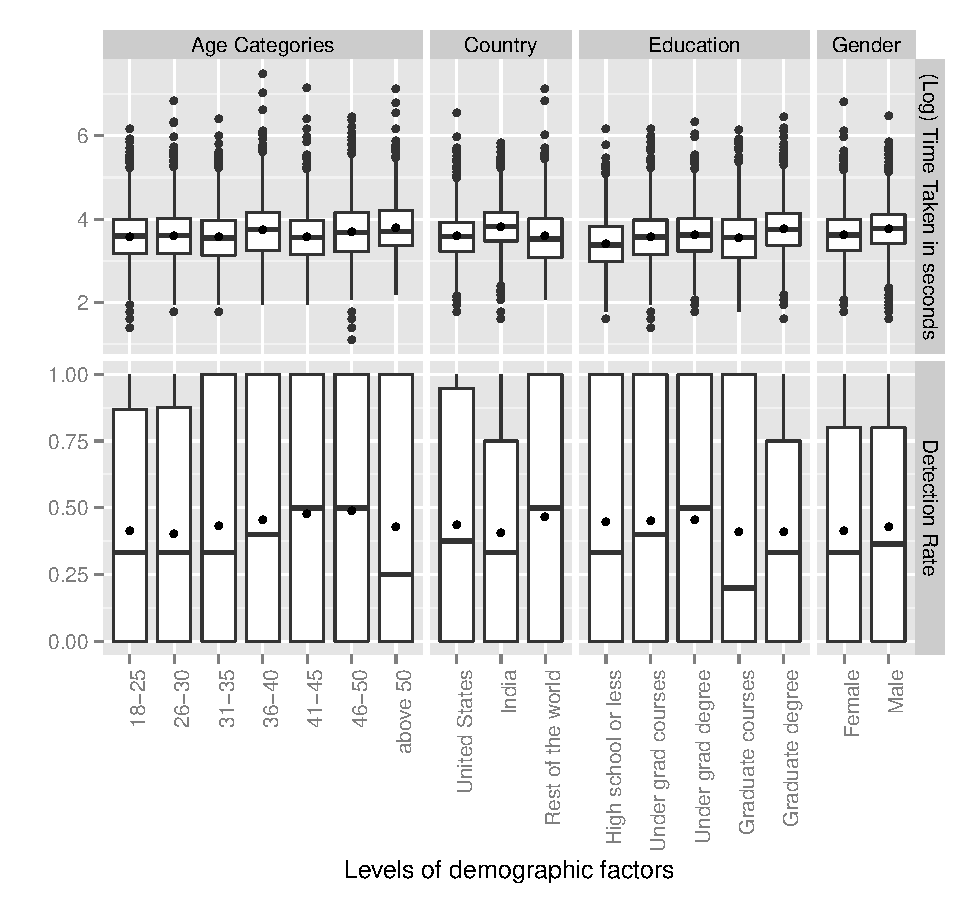
\includegraphics[width=4in]{demographic_effect.pdf} 
   \caption{Boxplots of average log time taken and proportion correct responses (detection rate) of all the lineups plotted for each demographic factor levels. The dots inside the boxes represent means. Some differences in means of various demographic factors are observed. Variability in detection rate indicates large variability in lineup difficulties. }
   \label{fig:demographic_effect}
\end{figure}


In Table~\ref{tbl:model_result_demographics} notice that lineup specific error is estimated as 2.27 which is much higher than any of the other parameter estimates in the model. This indicates that the major and most important factor affecting the detection rate is  lineup difficulty.  So although the demographic factors emerge from the model to be statistically significant, the practical significance is minimal. We illustrate this with the following example of graduate degree.

While some of the demographic factors are strongly statistically significant, the main source of variation in detection rate is the lineup difficulty. For example, let's examine the effect of an undergraduate degree. To see just how large the effect is, we examine the change in detection rate for a (hypothetical) 18-25 year old female in the United States, with some graduate course work as compared to an undergraduate degree, for an average difficulty lineup (random effect of zero). Plugging in the relevant quantities to the fitted model gives a difference equal to:
$$ \frac {\exp(-0.63-0.13)}{1+\exp(-0.63-0.13)}-  \frac {\exp(-0.63+0.16)}{1+\exp(-0.63+0.16)} = 0.319- 0.385 =-0.066.$$ 

The person with some graduate course work picks the data plot  on average in 31.9\% of lineups of average difficulty, as compared to 38.5\% if they have an undergraduate degree. This difference is reduced to 4\% for a lineup with one standard deviation order of magnitude difference in difficulty. For two standard deviations it further reduces to 0.6\%. Thus, although there is a statistically significant difference in the proportion at which participants identify the  data plot for some demographic factors, these are not  significant in any practical sense.  Figure~\ref{practical_impact_und_und_graduate.pdf} illustrates this example showing fitted models for a US 18-25 female with either a high school education or an undergraduate degree.  Similar calculations show the same negligible impact of age level 36-40 (0.068 at most)  and country India (-0.042 at most) on the probability of a correct response. Thus even though some of the demographic factors are statistically significant, practically, demographics do not substantially influence the results. 

\begin{figure}[htbp] 
   \centering
    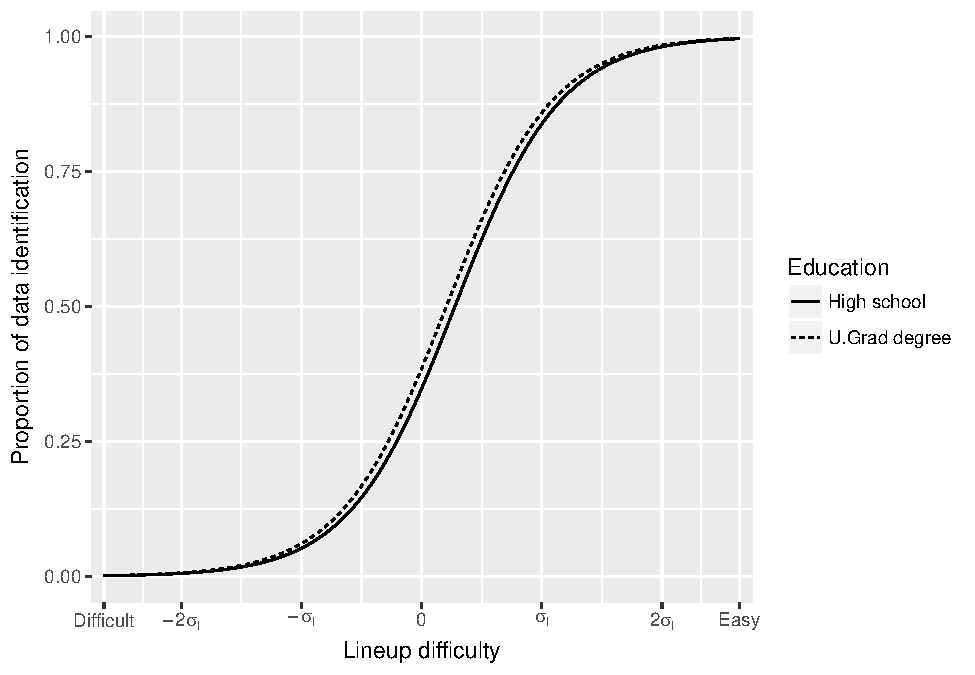
\includegraphics[width=3.2in]{practical_impact_und_graduate.pdf} 
    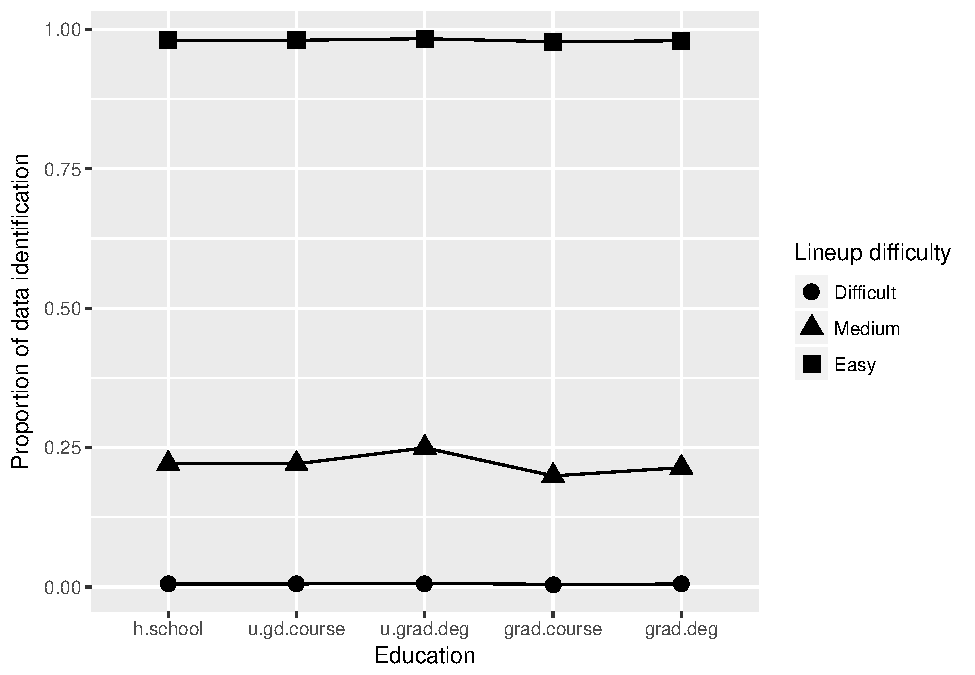
\includegraphics[width=3.2in]{practical_impact_degree.pdf} 
   \caption{Proportion of estimated data identifications by an 18-25 year old female in the United States with an under graduate degree compared to a high school degree. Even though having an under graduate degree leads to  statistically significant increase, the effect size in the dependent variable is  0.04 which is  negligible from a practical point of view. The difference diminishes as we move away one or two standard deviations ($\sigma_{\ell} = 2.27$) 
   of lineup variability.}
   \label{practical_impact_und_und_graduate.pdf}
\end{figure}




\subsection{Learning Trend} Models \eqref{eqn:trend_response} and \eqref{eqn:trend_time} are fitted to the data from experiments~5,~6, and~7 separately. Each participant evaluated 10 lineups in 10 attempts. In this model, attempt is fitted as a factor variable to allow for all possible non-linear learning trends.  It should be noted that we also examined an alternative to model~\eqref{eqn:trend_response} where attempt was linearly fitted as a continuous covariate, but this also was not significant.

The parameter estimates and $p$-values of the fixed effects from model~\eqref{eqn:trend_response} are presented in Table~\ref{tbl:model_result_response} in the Appendix~\ref{sec:exp_design}. Only for experiment~6 there is some evidence of a learning curve. There are marginally small $p$-values for most of the attempt levels, and positive parameter estimates, suggesting that more attempts increases detection rate. 


To visualize how  detection rates change over successive attempts, we fitted model~\eqref{eqn:trend_response} excluding the covariates related to attempt from the model and computed the residuals. Least square regression lines were fitted through the subject specific residuals as shown in Figure~\ref{fig:learning_trend_response}. The averages of these residuals for each of the attempts are shown as dots. Two important features were observed; one is subject specific variability and the other is random slope with attempts which indicates subjects specific learning trend. Some subjects show improvement over time and some show the decrease in performance. Although, the model fit experiment~6 suggested a statistically significant learning curve the plots indicates that it is minimal. 

\begin{figure}[htbp] 
   \centering
    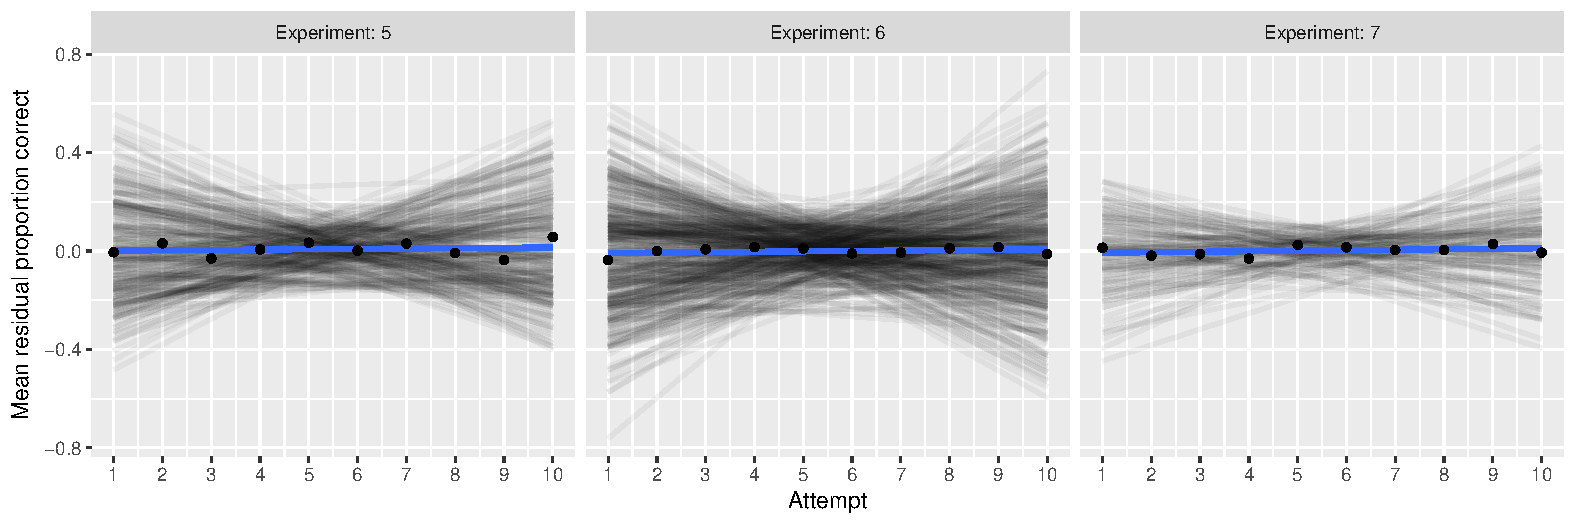
\includegraphics[width=6.3in]{learning_trend_subject.pdf} 
   \caption{ Least square lines fitted through the subject specific residual proportion correct obtained from model~\eqref{eqn:trend_response} fitted without attempt are plotted against attempt. Subject specific positive and negative slopes are observed. Mean residuals are shown as dots and least square regression lines fitted through the points show no overall learning trend in each of the three experiments.}
   \label{fig:learning_trend_response}
\end{figure}


Table~\ref{tbl:model_result_time} in the Appendix~\ref{sec:exp_design} presents the results of model~\eqref{eqn:trend_time} where response time is examined with respect to attempt. Attempt is modeled as a linear covariate here, with a shift factor used to adjust for additional time on the first lineup evaluated. Interestingly, time to respond significantly decreases as number of attempts increases, for all three experiments. 
The parameter $\alpha$ for fixed effect covariate attempt is highly significant in all the experiments. The negative estimates suggest that on average later attempts took less time. Even though observers did not improve in their performance in successive attempts, they became more efficient in their response. The parameter $\alpha_1$ for first attempt is also highly significant. The positive estimates of $\alpha_1$ indicates that first attempt made by an observer required much more time than any of the other attempts. One explanation might be that participants take the chance to  carefully read through instructions and familiarize themselves  with the types of plots used in the experiment before evaluating their first lineup, which would inflate the time taken on the first lineup. Each of the experiments asks observers to give a reason for their choice (out of a list of pre-defined answers. For each lineup evaluation, participants are also asked to state how confident in their choice they are (on a scale of 1 to 5).  Later pages of the web site were identical  except for the lineup. 


To visualize how the time taken reduces over the successive attempts, we fitted model~\eqref{eqn:trend_time} excluding the covariate attempt from the model and computed the residuals. Least square regression lines are fitted through the subject specific residuals. Subject specific slopes are much different in each of the three experiments as we see in Figure~\ref{fig:learning_trend_time}. Some subjects improved over attempts by taking less time in the later attempts while others got worse. The averages of these residuals for each attempt are plotted as dots. Least square regression lines are fitted to these points excluding the first attempt since for first attempt we fitted an indicator covariate. The downward trends are evident in the plots. All the slopes are highly significant. As expected we observed large positive residuals for each of the experiments for first attempt. 


\begin{figure}[htbp] 
   \centering
%   
\includegraphics[width=6.5in]{learning_trend_time.pdf}    
 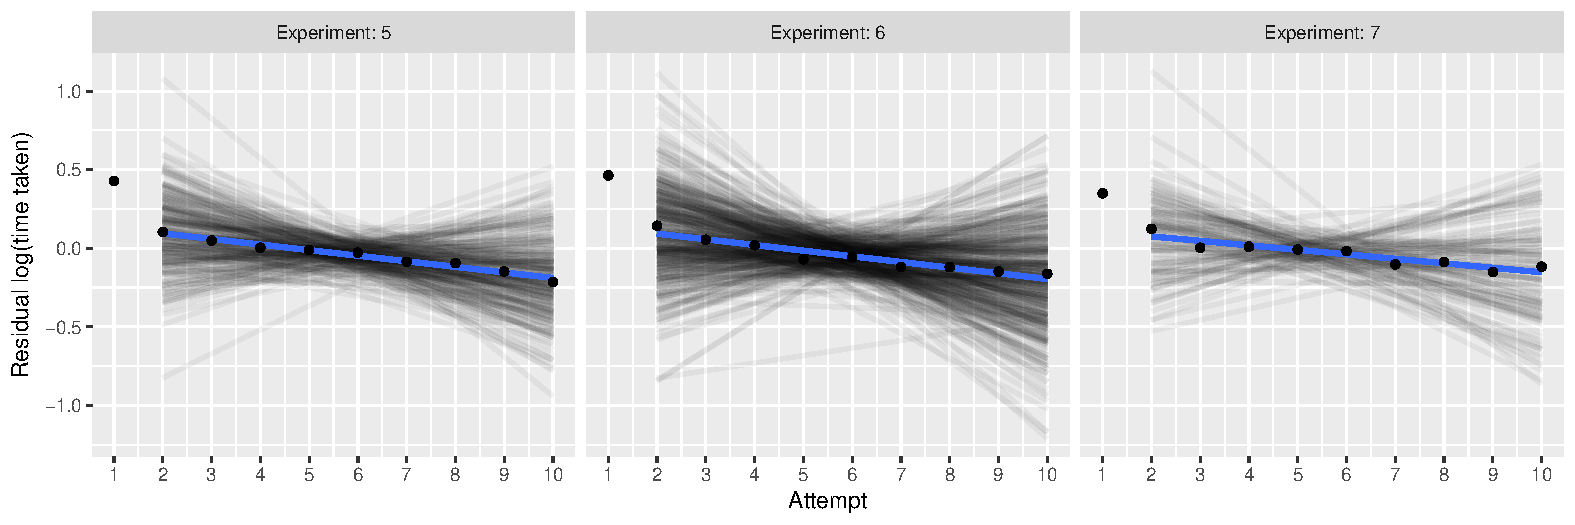
\includegraphics[width=6.3in]{learning_trend_time_subject.pdf}    
   \caption{Least square regression lines fitted through the subject specific residuals obtained by  fitting model~\eqref{eqn:trend_time} without covariate attempt. Differences in subject specific slopes are observed. Some of the subjects did worse over successive attempts while others did better. Averages of these residuals are plotted as dots and least square regression lines are fitted to obtain overall trends. For all the three experiments the overall downward slopes are statistically significant which indicates that MTurk workers become more efficient as they progress through their attempts.}
   \label{fig:learning_trend_time}
\end{figure}



% ===================================================================================
\section{Conclusion}
%------------------------------------------------------------------------------------

Human demographics have the potential to influence performance when the lineup protocol is used for statistical inference. In our study of the demographic effects on performance across a set of different experiments we found some statistically significant effects. Age group 36-40, people who have a graduate degree have a significantly higher detection rate. India shows significantly lower detection rate compared to United States. Gender does not have any significant effect. However, the effects are minimal, on the order of a few percentage points different from the average. These results are very important for the power of visual tests as they demonstrate the robustness of the test against different human factors.

Individual learning trend is observed in time taken but not so much in observer performance. Some individuals improved on their performances while others showed a decrease on successive attempts. This could be interpreted as good, in the sense that it means that observers could realistically be recruited from sources like MTurk, and that substantial training is not necessary in order to obtain useful evaluations of lineups in practice. However, we had hoped that lineups may be a useful teaching tool, to improve students ability to read data plots, and the lack of a learning trend diminishes this idea, at least for short term learning. 

There are many more ways that the lineup protocol might be tested to learn what we might expect about its performance for tackling real data mining problems. Possible changes in the lineup protocol in the pipeline are allowing observers to select more than one plot, and to vary the size of the lineup from 20 to a smaller number, and have observers all see different lineups with different null sets.  This paper assessed the effect of human factors on the experiments conducted to date. As changes to the lineup protocol are suggested by other experiments the human factor effects may need to be examined again.


\if1\blindDoc
{
%------------------------------------------------------------------------------------
\paragraph{Acknowledgments}
%------------------------------------------------------------------------------------
This work was funded in part by National Science Foundation grant DMS 1007697. All studies were conducted with approval from the Institutional Review Board IRB 10-347.
} \fi


\bibliographystyle{asa}
\bibliography{references}



% ---------------------------------------- Appendix ----------------------------------

\appendix


% ===================================================================================
\section{Experimental Methods}\label{sec:exp_design}
%------------------------------------------------------------------------------------

Two of the factors, signal in the data and individual abilities, were studied in \cite{majumder:2013}. The choice of visual test statistic was examined in \cite{heike:2012}. In each of these analyses demographic factors were given a cursory glance, to ensure that they did not have large effects on the results. The design of experiments 5, 6 and 7 enables the examination of learning trend, which is studied in this paper. Experiment~9 was a real test case for visual statistical inference, and in order to understand the significance of the structure in the genomic data, multiple lineups were made in which location of the actual data plot, and the sample of nulls, were randomized. This enables the assessment of the effect of these factors on the results. This section describes the experimental methods used to examine the effects of demography, sample of null plots and the existence of a learning trend. 

\subsection{Demographic Factors}
\noindent
For all  ten experiments shown in Table~\ref{tbl:visual_stat}, the following demographic information was collected from subjects:

\begin{enumerate} \leftmargin 5cm  \itemsep 0in
\item {\it Age group}, with categories set to be 18-25, 26-30, 31-35, 36-40, 41-45, 46-50, above 50.
\item {\it Gender}, male or female.
\item {\it Education level}, with levels being high school or less, some undergraduate courses, undergraduate degree, some graduate courses, and graduate degree.
\item {\it Geographical location}, collected from the IP address of the participants' computer, as latitude, longitude, city and country. 
\end{enumerate}


Let $Y_{ij}$ denote the response from observer $i$ on a lineup $j$, with $Y_{ij} =1$ if the actual data plot is chosen, otherwise $Y_{ij} =0$. The factors are examined in association with the observer's response using a logistic regression with random effect terms:

\begin{equation} \label{eqn:demographic_response}
g( \pi_{ij} )= \mu + \alpha_{k(i)} + \gamma_{l(i)} + \tau_{m(i)}+ \kappa_{s(i)} + \ell_j,  
\end{equation}

where $\pi_{ij}=  E(Y_{ij})$ is the probability that  observer $i$ picks the actual data plot from lineup $j$, $\mu$ is an overall population average, $\alpha$, $\gamma$, $\tau$ and  $\kappa$ are the effects of age group $k(i)$, gender $l(i)$, education level $m(i)$ and country name $s(i)$, respectively, for observer $i$. The term $\ell_j$ is a random intercept predicting lineup difficulty level and we assume independence and normality of the errors, i.e.\ $\ell_j \sim N(0, \sigma_\ell^2)$.  $g(.)$ denotes the {\it logit} link function $g(\pi)=\log(\pi) - \log(1-\pi); 0 \le \pi \le 1$.


Similarly, we model the  time  an observer takes to identify a panel from a lineup. Let $Z_{ij}$ denote the logarithm of time taken for  observer $i$ to evaluate  lineup $j$. Let $\mu_{ij}=  E(Z_{ij})$ be the average of the (log) time taken by  observer $i$ to pick a panel from lineup $j$. We model this in a mixed effects model of the same structure as model~(\ref{eqn:demographic_response}) given as:
%\hh{
\begin{equation} \label{eqn:demographic_time}
Z_{ij} = \mu + \alpha_{k(i)} + \gamma_{l(i)} + \tau_{m(i)}+ \kappa_{s(i)} + \ell_j+ \epsilon_{ij},  
\end{equation}
where $\mu$ represents overall average of log time taken by an observer to evaluate a lineup, $\alpha$, $\gamma$, $\tau$ and  $\kappa$ are as described in model~\eqref{eqn:demographic_response}, $\ell_j$ is a lineup-specific random effect for the time needed to evaluate a lineup, with $\ell_j \sim N(0, \sigma_\ell^2)$ and the overall error $\epsilon_{ij} \sim N(0, \sigma^2)$.  

\subsection{Learning Trend} Learning trend of a subject can be observed in terms of performance over successive responses when multiple lineups are shown for evaluation. Experiments 5, 6 and 7 were used for this. Each subject was shown a total of 10 lineups randomly selected from a pool of lineups. The lineups are not necessarily of the same difficulty level, but the order of lineups was randomized. The responses of the lineups were recorded by attempt 1 through 10. Attempt 1 means that the response is for the first lineup the observer evaluates and attempt 10 refers to the response for the 10th lineup. The goal is to estimate whether performance of the observer improves, or changes, from attempt 1 to attempt 10. 

It should be noted that we are examining the observer's performance, when we model response as detected or not, but this is not the goal of visual inference. Visual inference is constructed to measure the significance of structure discovered in data. It is expected that some observers will be more skilled at reading data plots, and hence, more readily detect the plot that is different. It is also expected that as observers gain experience in evaluating lineups that they become more proficient in reading data plots, particularly if feedback is given on whether the actual data plot was chosen or not. Choosing the actual data plot will be more difficult in some lineups than others, and indeed should happen purely by chance in some lineups. So in this context, detected, or not, is used as a response to examine individual differences. 

Let $Y_{ijk}$ denote the response from observer $i$ on lineup $j$ at their $k$th evaluation attempt, where $Y_{ijk}=1$ if the observer detected the actual data plot otherwise  $Y_{ijk}=0$. Let $\pi_{ijk}=  E(Y_{ijk})$ be the probability that  observer $i$ picks the actual data plot from lineup $j$ in their $k$th attempt. Learning trend is assessed using a generalized mixed effects model of the form
\begin{equation} \label{eqn:trend_response}
g( \pi_{ijk} )= \mu + \alpha_k + u_i +  a_{i} k + \ell_j,  
\end{equation}
where $\mu$ is an overall population average, $\alpha_k$ is the effect of the $k$th attempt on the probability, using the first attempt as reference, $\alpha_1 = 0$, and $k = 1, ..., K$, $u_i$ and $a_i$ are observer specific random effects, $i = 1, ..., I$. The term, $u_i$ is a random intercept, describing a basic subject-specific ability, with $u_i \sim N(0, \sigma_u^2)$. 
The term $a_i$ is a random slope capturing an individual's specific learning effect over the course of $K$ attempts, where $a_i \sim N(0, \sigma_a^2)$. 
For $\ell_j$ a normal distribution, $N(0, \sigma_\ell^2)$, is assumed, and $\ell_j$ is a random intercept predicting lineup difficulty level. $g(.)$ denotes the {\it logit} link function $g(\pi)=\log(\pi) - \log(1-\pi); 0 \le \pi \le 1$. The inverse link function, $g^{-1}(.)$, from equation~\ref{eqn:trend_response} leads to the estimate of the subject and the lineup specific probability of successful evaluation in the $k$th attempt by a single observer as 
\begin{equation} \label{eqn:trend_power}
\hat p_{ijk} =  g^{-1}(\hat{\mu} + \hat{\alpha}_k + \hat{u}_i +  \hat{a}_i k + \hat{\ell}_j).
\end{equation}

When time taken to evaluate a lineup is used as the response, let $Z_{ijk}$ denote the logarithm of time taken for an observer $i$ to evaluate a  lineup $j$ in his/her $k$th attempt. Let $\mu_{ijk}=  E(Z_{ijk})$ be the average of the (log) of time taken by  observer $i$ to choosing a  panel from lineup $j$ in his/her $k$th attempt. We evaluate this in a mixed effects model of the form

\begin{equation} \label{eqn:trend_time}
Z_{ijk} = \mu + \alpha_1 + \alpha k + u_i +  a_{i} k + \ell_j + \epsilon_{ijk},  
\end{equation}
where $\mu$ represents overall average of log time taken by an observer to evaluate a lineup, $\alpha$ is the average change in log time taken for each additional attempt,  $\alpha_1$ is an offset in log time taken for the first attempt. All other effects are random effects: $u_i$ is a subject-specific intercept representing individual speed of an observer with $u_i \sim N(0, \sigma_u^2)$, $a_i$ is a subject-specific slope representing the deviation of the speed-up (or -down) by attempt $k$, with $a_i \sim N(0, \sigma_a^2)$, $\ell_j$ is a lineup-specific random effect for the time needed to evaluate a lineup, $\ell_j \sim N(0, \sigma_\ell^2)$ and the overall error $\epsilon_{ijk} \sim N(0, \sigma^2)$.
Equation~\ref{eqn:trend_time} leads to the estimate of the subject and the lineup specific time taken for an evaluation in $k$th attempt by a single observer as 
\begin{equation} \label{eqn:trend_time_est}
\hat \mu_{ijk} =  \hat{\mu} + \hat{\alpha_1}+ \hat{\alpha}k + \hat{u}_i +  \hat{a}_i k + \hat{\ell}_j.
\end{equation}

To fit all these mixed effect models the function {\tt lmer()} is used from R package {\tt lme4} by \cite{lme4:2015, lme4:paper}. We employ a normal approximation to obtain $p$-values corresponding to fixed effect parameters estimates.  


\subsection{Data Collection Methods}  Human subjects were recruited to evaluate the experimental lineups through MTurk \citep{turk}.  It is an online work place where people from around the world can sign up for so-called `HIT's, human intelligence tasks, generally short tasks that are humans are typically better at solving than computers. Usually tasks are very simple and no specialized training is required to do them. Tasks are designed for anyone to do but some tasks may require some skills depending on the recruiters' need. %Each task is usually planned to completed in a short time.  
 For completing a HIT workers are paid a small amount of money, on the order of minimum wage in the USA. 


We designed and developed a web application which enables the display of lineups to  observers as per experimental need. The MTurk workers were re-directed to this web application to complete their assigned tasks. Responses were collected, stored automatically into a local database server, along with demographic information, age group, gender and education level. The time taken for each evaluation is computed based on the time the plot was shown and the time the feedback was received. Location of an observer is determined based on the ip address of the observer.





% ===================================================================================
\section{Some tables and figures}\label{sec:tbl_fig}
%------------------------------------------------------------------------------------

\begin{figure}[htbp] 
   \centering
   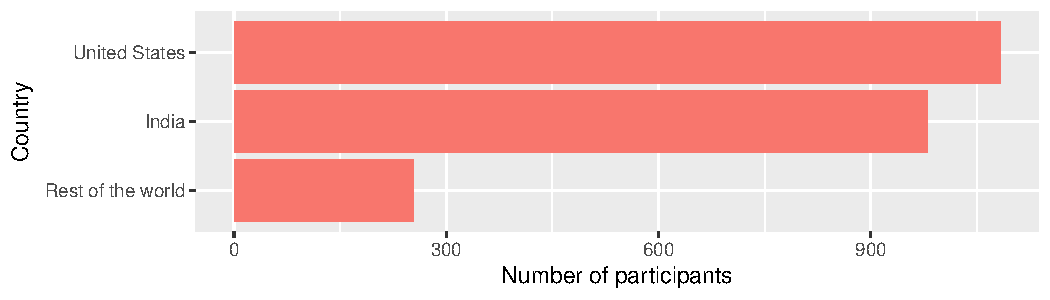
\includegraphics[width=4.5in]{turker_country.pdf} 
   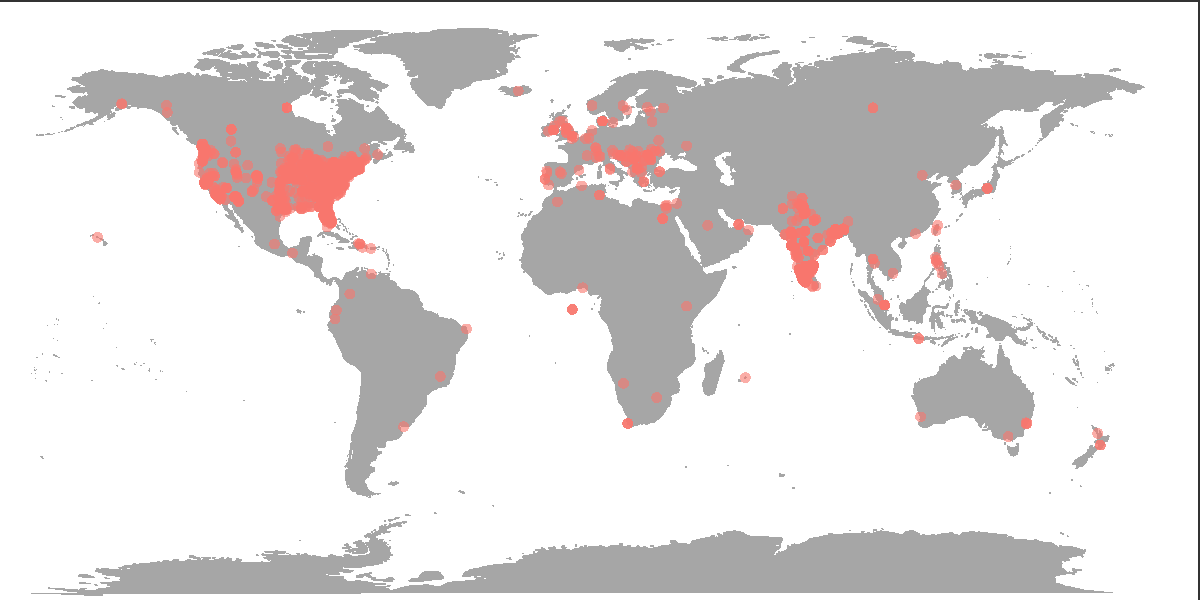
\includegraphics[width=4.5in]{turker_location.pdf}    
   \caption{Location of Amazon Mechanical Turk workers participating in the experiments. Most subjects came from India and the United States, but subjects from countries around the world took part.}
   \label{fig:turker_location}
\end{figure}

\begin{table}[hbtp]
\caption{\label{tbl:turker_location}Demographic information of the subjects participating in the MTurk experiments. Average time taken for evaluating a lineup is shown in seconds.}
\centering
\scalebox{.85}{
\begin{tabular}{rlrrcr}
  \hline
  && \multicolumn{2}{c}{Participants}&Average& Number of\\
  \cline{3-4}
 Factor & Levels & Total &\% & Time & Responses \\ 
  \hline
Gender & Female & 989 & 42.26 & 43.69 & 10538 \\ 
   & Male & 1351 & 57.74 & 48.75 & 13542 \\  
\hline
  Education & High school or less & 194 & 8.29 & 37.13 & 2253 \\ 
   & Under grad courses & 418 & 17.86 & 42.85 & 4068 \\ 
   & Under grad degree & 585 & 25.00 & 44.53 & 5792 \\ 
   & Graduate courses & 247 & 10.56 & 44.63 & 2471 \\ 
   & Graduate degree & 899 & 38.42 & 52.07 & 9496 \\ 
\hline
  Age & 18-25 & 743 & 31.75 & 43.50 & 7340 \\ 
   & 26-30 & 549 & 23.46 & 46.19 & 5610 \\ 
   & 31-35 & 375 & 16.03 & 44.19 & 3912 \\ 
   & 36-40 & 257 & 10.98 & 54.97 & 2714 \\ 
   & 41-45 & 140 & 5.98 & 43.89 & 1510 \\ 
   & 46-50 &  94 & 4.02 & 49.54 & 994 \\ 
   & above 50 & 184 & 7.86 & 52.32 & 2000 \\ 
\hline   
  Country & United States & 1086 & 46.41 & 39.65 & 10763 \\ 
   & India & 980 & 41.88 & 52.63 & 10238 \\ 
   & Rest of the world & 279 & 11.92 & 50.38 & 3079 \\ 
  
   \hline
\end{tabular}
}
\label{tbl:demographics}
\end{table}


% latex table generated in R 3.4.1 by xtable 1.8-2 package
% Wed Oct 18 17:43:02 2017
\begin{table}[ht]
\caption{\label{tbl:anova_factor}Analysis of variance (ANOVA) table comparing full model, all the demographic factors, with the reduced models, obtained by removing respective factor variable. Gender does not have a significant effect on detection rate, but does on time to respond. All factors significantly affect time to respond.}
\centering
\scalebox{0.9}{
\begin{tabular}{lrrrrlrrrr}
& \multicolumn{4}{c} {Log Time (model~\ref{eqn:demographic_time})} & &\multicolumn{4}{c} {Detection rate (model~\ref{eqn:demographic_response})}  \\
\cline{2-5} \cline{7-10} 
 & Deviance & $\chi^2$ & df & $p$-value && Deviance & $\chi^2$ & df & $p$-value \\ \cline{2-5} \cline{7-10}
Full  & 52609.1 & \multicolumn{1}{c}{---} & \multicolumn{1}{c}{---} & \multicolumn{1}{c}{---} &  & 24140.5 & \multicolumn{1}{c}{---} & \multicolumn{1}{c}{---} & \multicolumn{1}{c}{---} \\ 
 - Age & 52081.3 & 527.8 & 6 & $<$0.001 & \hspace{0.5cm} & 24113.2 & 27.3 & 6 & $<$0.001 \\ 
 - Country & 52245.5 & 363.6 & 2 & $<$0.001 &  & 24114.8 & 25.7 & 2 & $<$0.001 \\ 
 - Degree & 52498.7 & 110.4 & 4 & $<$0.001 &  & 24116.0 & 24.5 & 4 & $<$0.001 \\ 
 - Gender & 52540.3 & 68.8 & 1 & $<$0.001 &  & 24138.9 & 1.6 & 1 & 0.200 \\ 
\cline{2-5} \cline{7-10}
\end{tabular}}
\end{table}


% latex table generated in R 3.4.1 by xtable 1.8-2 package
% Wed Oct 18 23:54:25 2017
\begin{table}[hbtp]
\centering
\caption{\label{tbl:model_result_response}Parameter estimates of models \eqref{eqn:trend_response} fitted to data from three different experiments using detection rate as the response to assess learning trend. Attempt number is fitted as a factor to enable modeling any sort of non-linear learning trend. Only experiment~6 shows some evidence of a learning trend, with detection rate essentially increasing as attempts increase.}
\scalebox{.9}{
\begin{tabular}{rr>{(}r<{,}>{\hspace{-.1in}}l<{)}>{\hspace{-.15in}}l<{}cr>{(}r<{,}>{\hspace{-.1in}}l<{)}>{\hspace{-.15in}}l<{}cr>{(}r<{,}>{\hspace{-.1in}}l<{)}>{\hspace{-.15in}}l<{}}
\cline{2-5} \cline{7-10} \cline{12-15} 
& \multicolumn{4}{c} {Experiment~5} & &\multicolumn{4}{c} {Experiment~6} && \multicolumn{4}{c} {Experiment~7}\\
\cline{2-5} \cline{7-10} \cline{12-15} 
Effect & Est & 2.5\% & 97.5\% &  & \hspace{1cm} & Est & 2.5\% & 97.5\% &  & \hspace{1cm} & Est & 2.5\% & 97.5\% &  \\ 
\cline{2-5} \cline{7-10} \cline{12-15} 
Fixed \\
$\mu$ & -1.32 & -1.73 & -0.92 & *** &   & -0.16 & -0.46 & 0.13 &  &   & -1.73 & -2.81 & -0.66 & ** \\ [3pt]
  $\alpha2$ & 0.30 & -0.17 & 0.78 &  &   & 0.26 & -0.07 & 0.58 &  &   & -0.40 & -1.23 & 0.44 &  \\ 
  $\alpha3$ & -0.20 & -0.68 & 0.29 &  &   & 0.31 & -0.02 & 0.63 & . &   & -0.15 & -0.99 & 0.68 &  \\ 
  $\alpha4$ & 0.13 & -0.35 & 0.61 &  &   & 0.34 & 0.01 & 0.66 & * &   & -0.41 & -1.24 & 0.42 &  \\ 
  $\alpha5$ & 0.35 & -0.14 & 0.83 &  &   & 0.34 & 0.02 & 0.67 & * &   & -0.10 & -0.92 & 0.73 &  \\ 
  $\alpha6$ & 0.10 & -0.40 & 0.60 &  &   & 0.20 & -0.12 & 0.53 &  &   & 0.03 & -0.84 & 0.89 &  \\ 
  $\alpha7$ & 0.33 & -0.17 & 0.82 &  &   & 0.11 & -0.22 & 0.43 &  &   & -0.00 & -0.84 & 0.84 &  \\ 
  $\alpha8$ & -0.01 & -0.51 & 0.50 &  &   & 0.31 & -0.01 & 0.64 & . &   & -0.06 & -0.88 & 0.76 &  \\ 
  $\alpha9$ & -0.20 & -0.70 & 0.30 &  &   & 0.34 & 0.01 & 0.67 & * &   & 0.21 & -0.67 & 1.08 &  \\ 
  $\alpha10$ & 0.51 & 0.02 & 1.01 & * &   & 0.19 & -0.14 & 0.53 &  &   & -0.20 & -1.07 & 0.67 &  \\ 
  Random \\
  $\sigma^2_u$ & \multicolumn{5}{l}{\phantom{-}0.91}  & \multicolumn{5}{l}{\phantom{-}0.89} & 0.82   \\ 
  $\sigma^2_a$ & \multicolumn{5}{l}{\phantom{-}0.04}  & \multicolumn{5}{l}{\phantom{-}0.04} & 0.05   \\ 
  $\sigma^2_l$ & \multicolumn{5}{l}{\phantom{-}1.47}  & \multicolumn{5}{l}{\phantom{-}1.43} & 3.38   \\ \cline{2-5} \cline{7-10} \cline{12-15} 
\\
\hline
\multicolumn{10}{l}{Signif. codes:  *** $<$ 0.001 $\le$ ** $<$ 0.01 $\le$ * $<$ 0.05 $\le$ . $<$ 0.1 $\le$ ` ' $<$ 1}
\end{tabular}}
\end{table}


% latex table generated in R 3.4.1 by xtable 1.8-2 package
% Wed Oct 18 23:37:55 2017
\begin{table}[bhtp]
\caption{\label{tbl:model_result_time}Parameter estimates of model~\eqref{eqn:trend_time} fitted for log time taken to evaluate a lineup. Both fixed effects parameters of Attempt ($\alpha_1$ and $\alpha$) are highly significant for all three experiments~5,~6 and~7.}
\centering
\scalebox{0.9}{
\begin{tabular}{lr>{(}r<{,}>{\hspace{-.1in}}l<{)}>{\hspace{-.15in}}l<{}cr>{( }r<{,}>{\hspace{-.1in}}l<{)}>{\hspace{-.15in}}l<{}cr>{(}r<{,}>{\hspace{-.1in}}l<{)}>{\hspace{-.15in}}l<{}}
\cline{2-5} \cline{7-10} \cline{12-15} 
& \multicolumn{4}{c} {Experiment~5} & &\multicolumn{4}{c} {Experiment~6} && \multicolumn{4}{c} {Experiment~7}\\

\cline{2-5} \cline{7-10} \cline{12-15} 
\multicolumn{2}{c}{Effect \hfill Est} & 2.5\% & 97.5\% &  &  & Est & 2.5\% & 97.5\% & &  & Est & 2.5\% & 97.5\% & \\ 
  \cline{2-5} \cline{7-10} \cline{12-15}
\multicolumn{2}{l}{Fixed}\\
$\mu$ & 3.80 & 3.72 & 3.88 & *** &   & 3.89 & 3.83 & 3.96 & *** &   & 3.75 & 3.64 & 3.85 & *** \\ 
  $\alpha_1$ & 0.32 & 0.25 & 0.39 & *** &   & 0.34 & 0.28 & 0.40 & *** &   & 0.28 & 0.18 & 0.38 & *** \\ 
  $\alpha$ & -0.04 & -0.05 & -0.03 & *** &   & -0.04 & -0.05 & -0.03 & *** &   & -0.03 & -0.04 & -0.02 & *** \\ 
\multicolumn{2}{l}{Random}\\
  $\sigma^2_u$ & \multicolumn{5}{l}{\phantom{-}0.52}   & \multicolumn{5}{l}{\phantom{-}0.49}  & 0.37   \\ 
  $\sigma^2_a$ & \multicolumn{5}{l}{\phantom{-}0.03}  & \multicolumn{5}{l}{\phantom{-}0.05}   & 0.05   \\ 
  $\sigma^2_l$ & \multicolumn{5}{l}{\phantom{-}0.09}   & \multicolumn{5}{l}{\phantom{-}0.20}   & 0.24   \\
  $\sigma^2$ & \multicolumn{5}{l}{\phantom{-}0.46}   & \multicolumn{5}{l}{\phantom{-}0.50}  & 0.45  \\ 
   \cline{2-5} \cline{7-10} \cline{12-15}
\end{tabular}}
\end{table}




\begin{table*}[hbtp] 
\centering 
\caption{Overview of 10 different Turk experiments, from which data was collected to study human factor effects. All of the experimental data were used to estimate the effect of demographic factors (DF) on visual inference while three were suitable for assessing learning trend (LT) and location effect (LE) was possible to assess using just one specially designed study.} 
\begin{tabular}{m{.5cm}m{2.6cm}m{2cm}m{5.5cm}m{3cm}} 
\hline\hline 
 & Experiment &  Test Statistic  & Lineup question & Used in study of\\ [0.5ex] % inserts table %heading 
\hline 
1  & Box plot & \begin{minipage}[t]{2cm} \begin{center}	\scalebox{0.12}{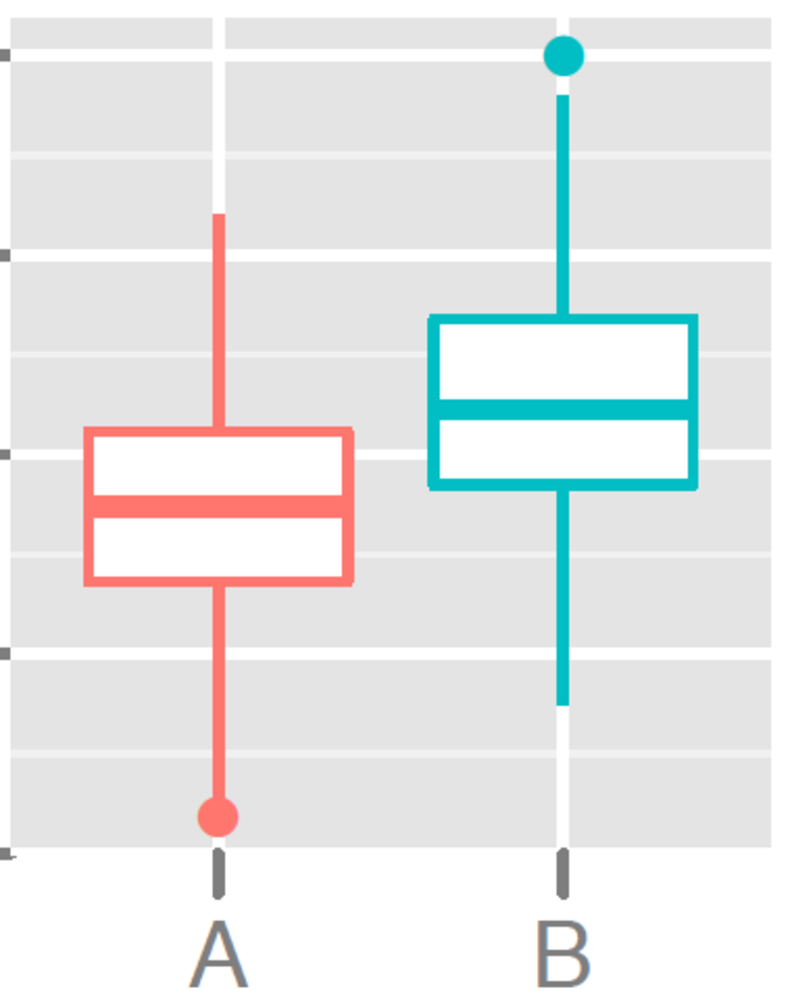
\includegraphics{stat_category1.pdf}} \end{center} \end{minipage} & Which set of box plots shows biggest vertical difference 
between group A and B? & DF\\
2 &  Scatter plot & \begin{minipage}[t]{2cm}  \begin{center} \scalebox{0.3}{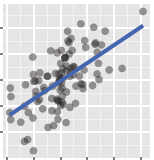
\includegraphics{stat_beta_k1.png}} \end{center} \end{minipage} & Of the scatter plots below which one shows data that has steepest slope? & DF\\
  3 & Contaminated plot &\begin{minipage}[t]{2cm} \begin{center} \scalebox{0.5}{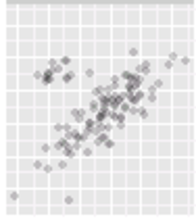
\includegraphics{stat_contaminated.pdf}} \end{center} \end{minipage} & Of the scatter plots below which one shows data that has steepest slope? & DF\\
 4 & Polar vs Cartesian & \begin{minipage}[t]{2cm} \begin{center}  \scalebox{0.32}{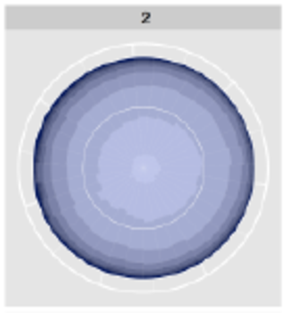
\includegraphics{stat_polar.pdf}} \end{center} \end{minipage} &Which plot is different?& DF\\
  5 & Hist vs density & \begin{minipage}[t]{2cm} \begin{center}  \scalebox{0.38}{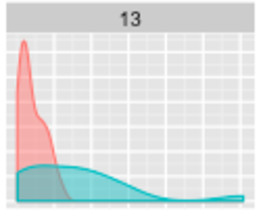
\includegraphics{stat_density.pdf}} \end{center} \end{minipage} &In which plot is the blue group furthest to the right?&  DF \hfill LT \hfill \phantom{.} \hfill \phantom{.} \\  
  6 & Violin vs boxplot & \begin{minipage}[t]{2cm} \begin{center}  \scalebox{0.35}{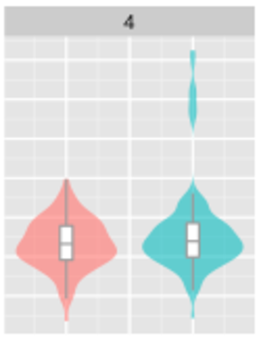
\includegraphics{stat_violin.pdf}} \end{center} \end{minipage}&  In which plot does the blue group look the most different from  the red group? &  DF  \hfill LT \hfill \phantom{.} \hfill \phantom{.} \\
  7 & Group separation & \begin{minipage}[t]{2cm} \begin{center}  \scalebox{0.4}{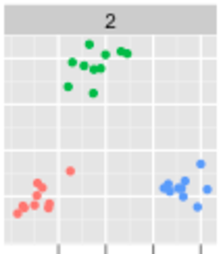
\includegraphics{stat_separation.pdf}} \end{center} \end{minipage} &Which of these plots has the most separation between the coloured groups? & DF  \hfill LT \hfill \phantom{.} \hfill \phantom{.} \\ 
  8 & Sine Illusion & \begin{minipage}[t]{2cm} \begin{center}  \scalebox{0.28}{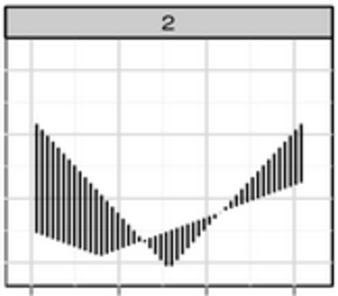
\includegraphics{stat_sine.pdf}} \end{center} \end{minipage} & In what picture is the size of the curve most consistent? & DF\\ 
  9 & Gene expression &\begin{minipage}[t]{2cm} \begin{center}  \scalebox{0.45}{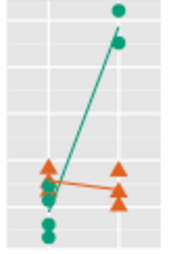
\includegraphics{stat_gene.pdf}} \end{center} \end{minipage} & In which of these plots is the green line the steepest, and the spread of the green points relatively small? & DF  \hfill \phantom{LT} \hfill {LE} \hfill \phantom{.}\\ 
  10 & Test normality & \begin{minipage}[t]{2cm} \begin{center}  \scalebox{0.35}{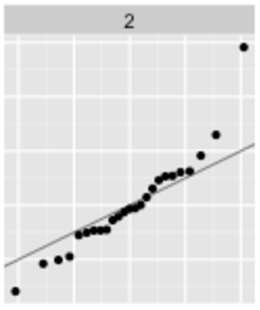
\includegraphics{stat_normality.pdf}} \end{center} \end{minipage} &Which of these plots is most different from the others? & DF\\ 

\hline 
\end{tabular} 
\label{tbl:visual_stat} 
\end{table*} 


\end{document}


